\documentclass[conference]{IEEEtran}
\IEEEoverridecommandlockouts
\usepackage{cite}
\usepackage{amsmath,amssymb,amsfonts}
\usepackage{algorithmic}
\usepackage{graphicx}
\usepackage{textcomp}
\usepackage{xcolor}
\usepackage[draft]{hyperref}

\selectcolormodel{cmyk}

\usepackage{tikz, pgfplots}
\usetikzlibrary{calc}
\usetikzlibrary{pgfplots.groupplots}
\usetikzlibrary{plotmarks}

\usepackage{ifthen}
\usepackage{xargs}

\def\BibTeX{{\rm B\kern-.05em{\sc i\kern-.025em b}\kern-.08em
T\kern-.1667em\lower.7ex\hbox{E}\kern-.125emX}}
\begin{document}

    \title{Increasing the Upper Bound for the EvoMan Game Competition}

    \author{\IEEEauthorblockN{Gabriel-Codrin \textbf{Cojocaru}}
        \IEEEauthorblockA{\textit{Faculty of Computer Science} \\
            \textit{``Al. I. Cuza'' University}\\
            Iasi, Romania \\
            gabriel.cojocaru@info.uaic.ro}
          \and
          
          \IEEEauthorblockN{Sergiu-Andrei \textbf{Dinu}}
          \IEEEauthorblockA{\textit{Faculty of Computer Science} \\
            \textit{``Al. I. Cuza'' University}\\
            Iasi, Romania \\
            sergiu.dinu@info.uaic.ro}
      
        \and
        \IEEEauthorblockN{Eugen \textbf{Croitoru}}
        \IEEEauthorblockA{\textit{Dept. of Computer Science} \\
          \textit{``Al. I. Cuza'' University}\\
          Iasi, Romania \\
          eugennc@uaic.ro}
      }

    \maketitle

    \begin{abstract}
      This paper describes a comparison between algorithms for evolving agents able to play the game Evoman.
      Our team took part in the ``Evoman: Game-playing Competition for WCCI 2020'', and won second place;
      beyond finding a good agent to satisfy the requirements of the competition - which aim at a good ability to generalise -,
      we have surpassed the existing non-general, best-known upper-bound.
      We have managed to exceed this upper bound with a Proximal Policy Optimization(PPO) algorithm, by discarding the competition requirements to generalise.
      We also present our other exploratory attempts: Q-learning, Genetic Algorithms, Particle Swarm Optimisation, and their PPO hybridizations. 
      Finally, we map the behaviour of our algorithm in the space of game difficulty, generating plausible extensions to the existing upper-bound.
    \end{abstract}

    \begin{IEEEkeywords}
        game-playing agent, Artificial Intelligence, EvoMan, Genetic Algorithm, Reinforcement Learning,
        Q-learning, Neuroevolution, Particle Swarm Optimization, Proximal Policy Optimization
    \end{IEEEkeywords}


    \section{Introduction}\label{sec:introduction}
    This paper contains our improvement on the upper-bound for playing the 2D shooting / platformer game Evoman\cite{evoman}.
    Our team took part in the ``Evoman: Game-playing Competition for WCCI 2020''\cite{evoman_competition}. While placing second\cite{evoman_competition_results}, we have managed to exceed the best-known upper-bound. This difference is due to the competition requirements for generalisation; the upper-bound has been provided by the organisers by dropping such requirements, and only by doing the same could we exceed it.

    Our initial exploratory attempts focused on an ensemble, $2$-stage cascade method. The first stage, designed to find good candidate solutions quickly, was either a Q-Learning\cite{q_learning}, a Genetic Algorithm\cite{genetic_algorithm} or Particle Swarm Optimization\cite{pso} algorithm. The candidate solutions are weights on a fixed-structure Artificial Neural Network, which plays the Evoman game. The second stage, aimed at further refining the solutions found by the first stage, is a slower Proximal Policy Optimization (PPO)\cite{ppo} algorithm.

    However, a simple random initialisation outperforms any of the first-stage algorithms, and the later experiments use PPO alone.

    The competition required the algorithm to train with half the opponents in the game, and to test with all of them. Our method shows significant overfit in this challenge. However, its otherwise good performance makes it appropriate for setting a new upper bound, since the upper bound is being computed individually, by training and testing against each opponent in the Evoman game.

    All datapoints from our research are arithmetic averages of $30$ repeats.

    \section{Problem Description}\label{sec:problem-description}

    \subsection{Environment}\label{subsec:environment}

    Evoman\cite{karinemiras,evoman} is a framework for testing competitive game-playing agents.
    This framework is inspired by Mega Man II\cite{capcom}, a game created by Capcom.
    Evoman is a 2D shooting game where the player controls an agent playing against an opponent.
    The agent will collect information about the environment through 20 sensors (Fig. 1):
    \begin{itemize}
        \item 16 correspond to horizontal and vertical distances to a maximum of 8 different opponent projectiles.
        \item 2 correspond to the horizontal and vertical distance to the enemy.
        \item 2 describe the directions the player and the enemy is facing
    \end{itemize}
    \begin{figure}
        \centering
        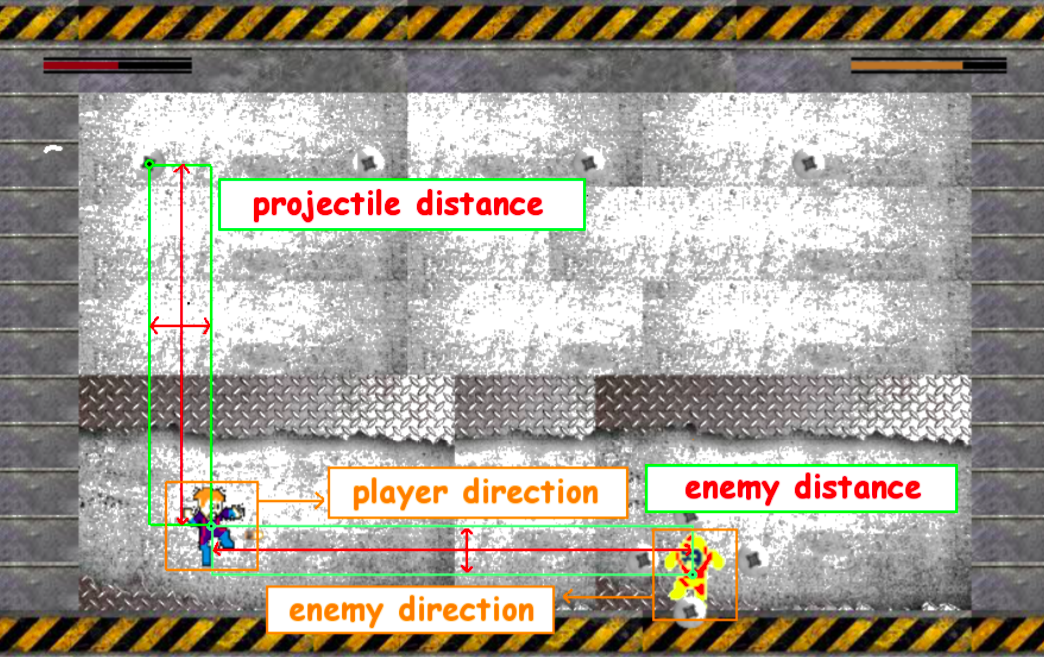
\includegraphics[width=0.5\textwidth]{images/Evoman3.png}
        \caption{Sensors available for the player\cite{evoman}.}
        \label{fig:sensors}
    \end{figure}
    The 5 actions which the agent may take are: walk left, walk right, shoot, press jump, release jump.

    The player and opponent start with 100 life points. On each hit received, their life points decrease.
    The player wins by reducing the opponent's life points to $0$, and lose if their life points are reduced to $0$ first.

    In the original Capcom game, the player would have to beat $8$ opponents and acquire their weapons
    once they are defeated.
    The additional difficulty of EvoMan comes from the fact that the player has to defeat all
    the opponents using only the starting weapon.
    Each opponent can be fought at a specific difficulty level.
    The difficulty level is an integer greater or equal than $1$ which is translated into a factor for the damage
    taken and damage given by the player; the higher the difficulty level the lower the damage given, and the higher the damage taken.
    The framework is freely available\footnote{\url{https://github.com/karinemiras/evoman_framework}}.
    There is also an extensive documentation
    available\footnote{\url{https://github.com/karinemiras/evoman_framework/blob/master/evoman1.0-doc.pdf}}.


    \subsection{Problem}\label{subsec:problem}
    How well an agent performs against an enemy is measured by how much damage they inflict, and how much damage to themselves they avoid - or, conversely, how much life points they have remaining, and how much life points the opponent has at the end of the game:
    \vspace{-0.1cm}
    \begin{gather*}
      gain = 100.01 + player\_life - enemy\_life \hspace{1cm} (1)
    \end{gather*}

    As both start with $100$ life points, the best possible value for gain is $200.01$, for a player which defeats the opponent without getting hit.

    The best known gain was $185.67$ (as a harmonic average of $8$ values, each for one of the $8$ opponents)
    \cite{evoman} and was obtained with a NEAT\cite{neat} algorithm. It is this value we've tried to exceed.\\

    There are also various levels of generalisation available; the least is training a single agent on a single opponent, as the above method does. The next is training a single agent on all opponents: instead of having $8$ specialised models for each opponent, a single unified model, trained on all $8$, could be attempted. Furthermore, we could train a single agent on a subset of the $8$, and test that agent on the full $8$. The competition\cite{evoman_competition} allowed free choice of $4$ training agents, and testing against all $8$.

    Another level of generalisation is learning from one difficulty level and applying to the others. While seeing this possibility, we did not attempt such a task, due to the current high difficulty of the problem.
    
    \section{Approach}\label{sec:approach}
    Our initial intention was to develop a cascade ensemble method where a fast algorithm could provide a better starting point to a slower algorithm.
    We expected the classic Q-learning\cite{q_learning} algorithm to quickly obtain a decent gain. Two more exploratory algorithms we have considered are Genetic Algorithms\cite{genetic_algorithm} and Particle Swarm Optimisation\cite{pso}. For our algorithmic parameters, we chose widely-used starting values, performing small-scale experiments to fine-tune them.
    
    The slower algorithm, intended to exploit the starting points provided by the first algorithm in the cascade, is a Proximal Policy Optimization\cite{ppo} algorithm. 

    To find the best first-stage algorithm we have made the following changes (which had no impact in the training and testing for the final solution to the problem, other than guiding the choice of algorithm):
    \begin{itemize}
        \item we have increased the difficulty from the default 2 up to 5.
        \item the evaluation is made only on the second opponent due to the varied environment.
        \item the gain function was modified as in Karine Miras' analysis\cite{evoman_blog} to:
        \begin{gather*}
          fitness = 
            0.9 \cdot (100 - enemy\_life) + 0.1 \cdot player\_life\\
            -\hspace{0.2cm} ln(nr\_of\_game\_timesteps) \hspace{1cm} (2)
        \end{gather*}
    \end{itemize}

    The best possible value for the fitness is $100$.

    The best exploratory algorithm would be trained on four enemies and
    used in cascade with PPO, without the changes mentioned in this section.

    \subsection{Solution structure}
    In all cases, a candidate solution is a fixed-structure feedforward Artificial Neural Network.

    The input and output layers are determined by the game framework. Each game frame gives us $20$ sensor values, and we also remember the past $2$ frames, alongside the movements we've made. Thus, $3 \cdot 20 + 2 = 62$ inputs. The ANN has $5$ outputs, corresponding to the $5$ actions accessible to the agent.

    We've decided on two hidden layers. At first, we've used $32$ perceptrons on each, but later extended to $64$ (only when using PPO). We haven't increased the number of perceptrons or hidden layers further, since our main issue proved to be overfit, not the ANN's inability to properly approximate the required function\cite{cybenko}.
    The activation function used is the Logistic Sigmoid; each layer has l2 regularisation applied to it, and each weight has a decay of $0.01$.
    The weights are initialised in the range $[-2, 2]$, with a minimum precision of $6$ decimal paces.
    
    
    \subsection{Q-Learning}\label{subsec:q-learning}
    We used a classic Q-Learning ANN to predict the reward function for each possible move.
    After each predicted move, we update the neural network using backpropagation. We compute the reward as the difference between the current score and the previous score:
    
    $ (prev\_enemy\_life - curr\_enemy\_life) \cdot 0.8 + (curr\_player\_life - prev\_player\_life) \cdot 0.2 $
    
    We have trained the agent on $5000$ games.
%    The (arithmetic) average number of frames per game for the best model is $287$.

    \subsection{Sparse Reward Genetic Algorithm}
    The second algorithm is a sparse reward Neuroevolution\cite{neuro} algorithm.
    The reward is defined as ``sparse'' because an agent doesn't find out how well it's doing until
    the end of the game, with no feedback during the game.
    An individual represents the binary encoding of the weights of a Neural Network.

    Since we are representing the individuals as bitstrings we were able to apply
    a Simple Genetic Algorithm\cite{genetic_algorithm}.

    %\pagebreak
    
    The configurations we have used for the GA are:
    \begin{itemize}
        \item population size: $50$
        \item number of generations: $500$
        \item crossover rate: $0.7$
        \item mutation rate: $\{0.008, 0.1\}$
        \item elitism: $1$ individual
    \end{itemize}
    We have tried $2$ experiments with different mutation rates in order to observe if a high
    mutation rate can lead to good results for the problem, since the role of this GA was
    chiefly exploratory in our ensemble. \\

    The solution of the GA is the best individual from the last generation.

    \subsection{Iterative Genetic Algorithm}
    The next algorithm is an iterative neuroevolution one.
    It is "iterative" because the agents are trained on a small number of game steps
    first, and then the number of game steps slowly increases. We've used this approach in order to save time; we believe it is reasonable to expect the initial agents to perform poorly, and thus require less time to decide on their quality.

    The fitness function is scaled based on the number of game timesteps in a way that an agent
    training on fewer timesteps will always have a fitness lower than an agent training on more timesteps.

    \subsection{Particle Swarm Optimization}\label{subsec:searching-neural-network-weights-with-particle-swarm-optimization}
    The configurations used for the PSO are:
    \begin{itemize}
        \item population size: $30$
        \item number of iterations: $200$
        \item cognitive weight: $\{0.4, 0.8, 1.5\}$
        \item social weight: $\{0.8, 0.4, 3\}$
        \item inertia weight: \{constant $1$, decreasing from $1$ by $0.0035$ every iteration\}
    \end{itemize}
    The same separation between sparse and iterative evaluations was made in the case
    of PSO, as was in the case of GA.

    \subsection{Proximal Policy Optimization}\label{subsec:proximal-policy-optimization}
    We have devoted significant computational resources to a PPO\cite{ppo}, expecting it to exploit and refine solutions.
    The configuration we have used for the PPO is:
    \begin{itemize}
        \item randomly initialized weights
        \item steps per epoch: $10000$
        \item epochs: $3000$
        \item gamma: $0.99$
        \item clip\_ratio: $0.2$
        \item pi\_lr: $3e-4$
        \item vf\_lr: $1e-3$
        \item train\_pi\_iterations: $80$
        \item train\_v\_iterations: $80$
        \item lambda: $0.97$
        \item target\_KL: $0.01$
    \end{itemize}

    \subsection{Particle Swarm Optimization Cascaded With Proximal Policy Optimization}\label{subsec:particle-swarm-optimization-cascaded-with-proximal-policy-optimization}
    The output weight configuration of an Artificial Neural Network resulting from a PSO search is the starting agent for PPO\@.
    While using the same PSO configuration as before, the ANN hidden layers size is increased from $32$ to $64$.
    
    \section{Experimental Investigation}\label{sec:experimental-investigation}

    The Q-learning algorithm serves as the starting point of our comparison.
    Even when trained and evaluated against the same opponent, it loses every game
    while inflicting almost no damage.

    The iterative GA leads to much better results than Q-learning (Fig.~\ref{fig:q_vs_ga_iterative}).
    We've also chosen a mutation probability of $0.008$. The results of the sparse GA and the iterative GA
    are not significantly different (Fig.~\ref{fig:overview}).

    Both PSO algorithms lead to much better results than either GA.
    The iterative PSO leads to worse results than the sparse PSO\@.
    In Fig.\ref{fig:overview} we can see that the best first-stage algorithm is the sparse PSO\@.
    
    We have tested PSO performance (Fig.~\ref{fig:pso_levels}), on multiple difficulties.

    
    \begin{figure}[!ht]
        \centering
        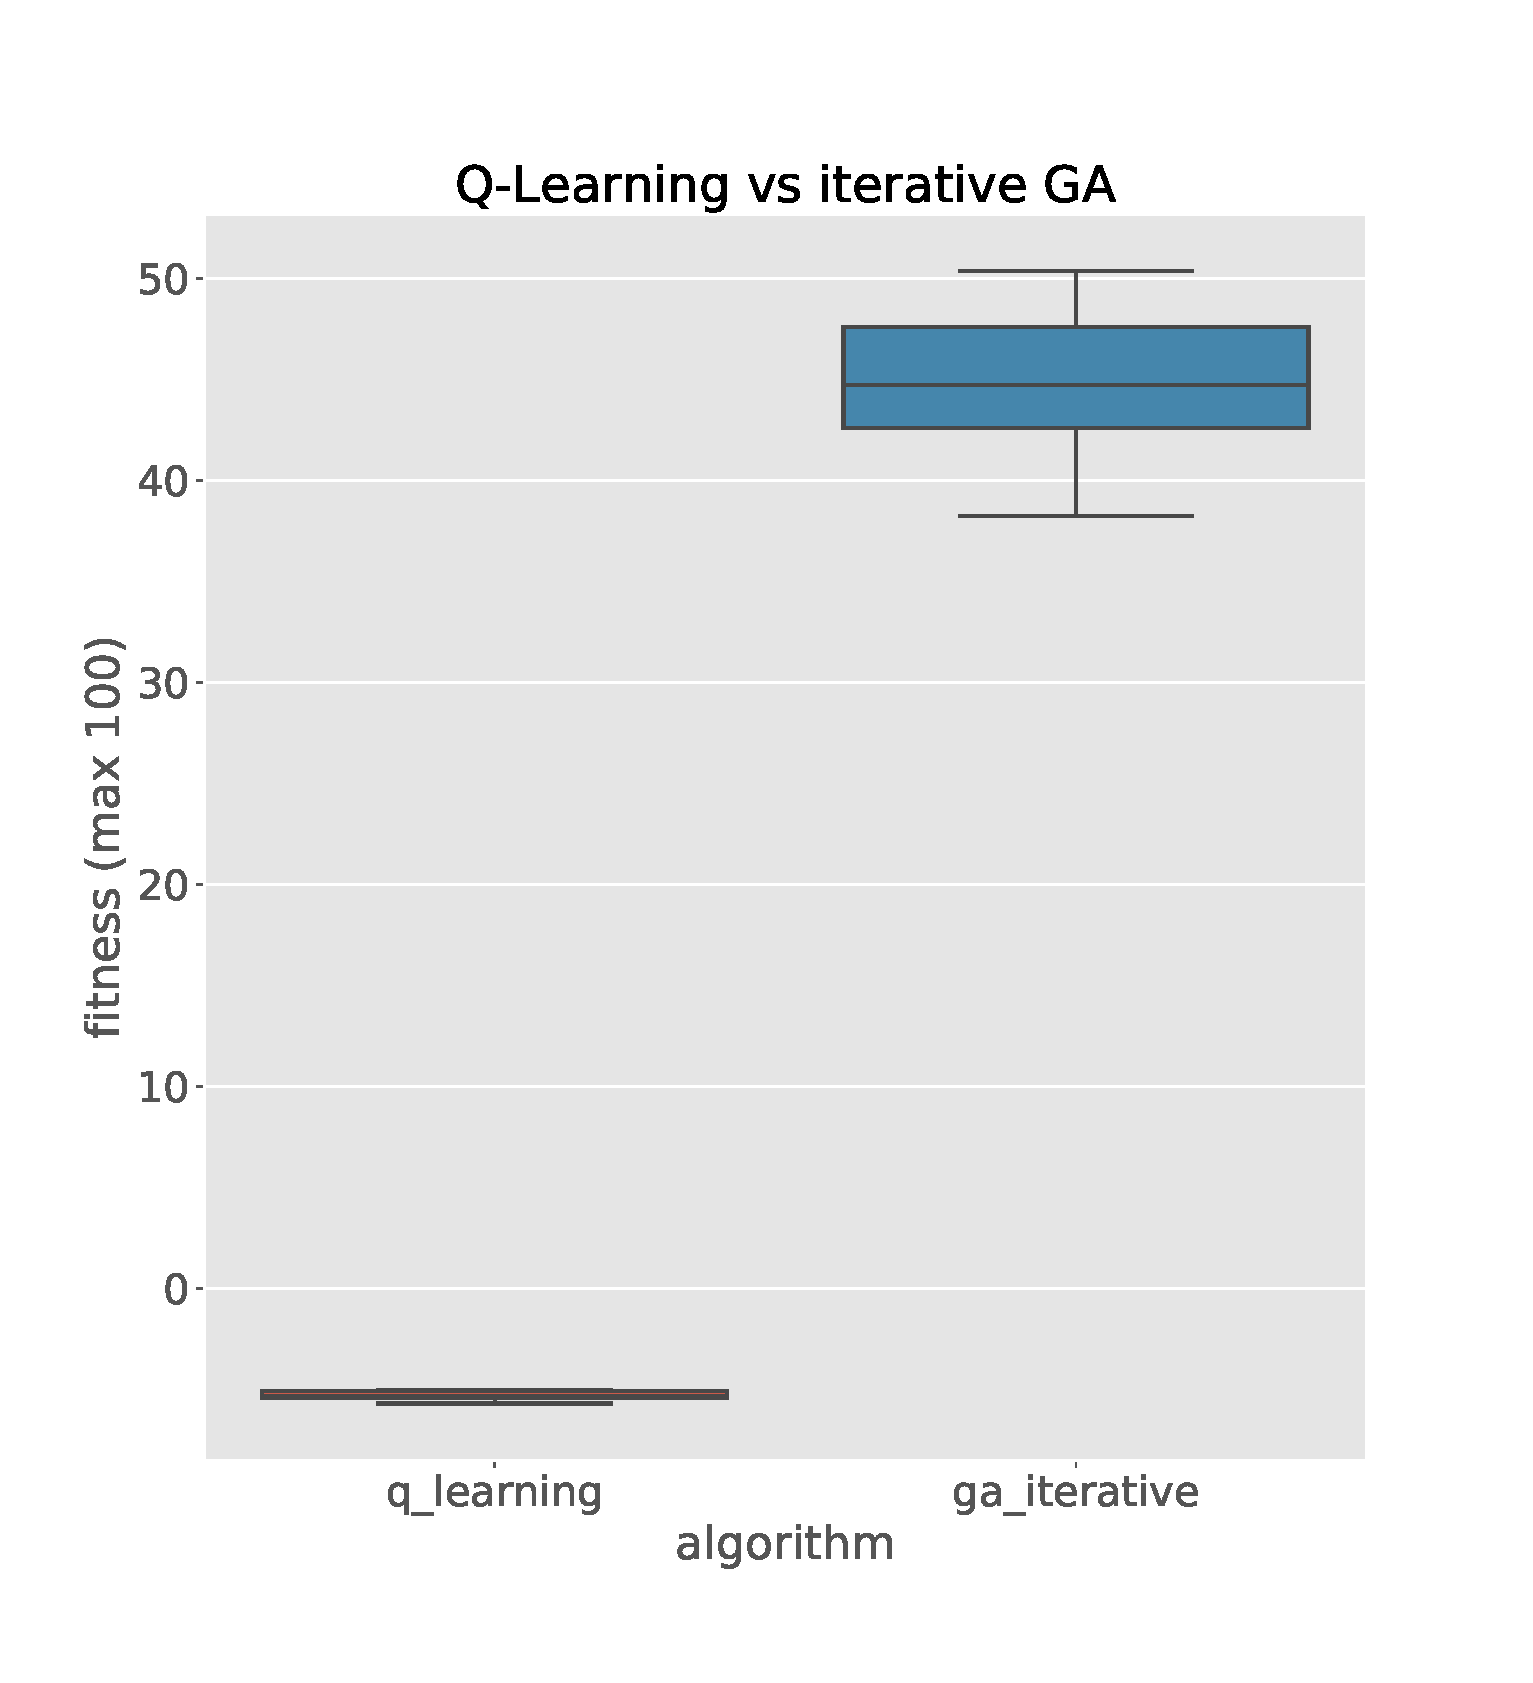
\includegraphics[width=0.5\textwidth]{old_images/q_vs_ga_iterative.eps}
        \caption{The fitness comparison between Q-learning and iterative genetic algorithms. Difficulty: $5$.}
        \label{fig:q_vs_ga_iterative}
    \end{figure}
      
    \pagebreak

    \begin{figure}[!ht]
        \centering
        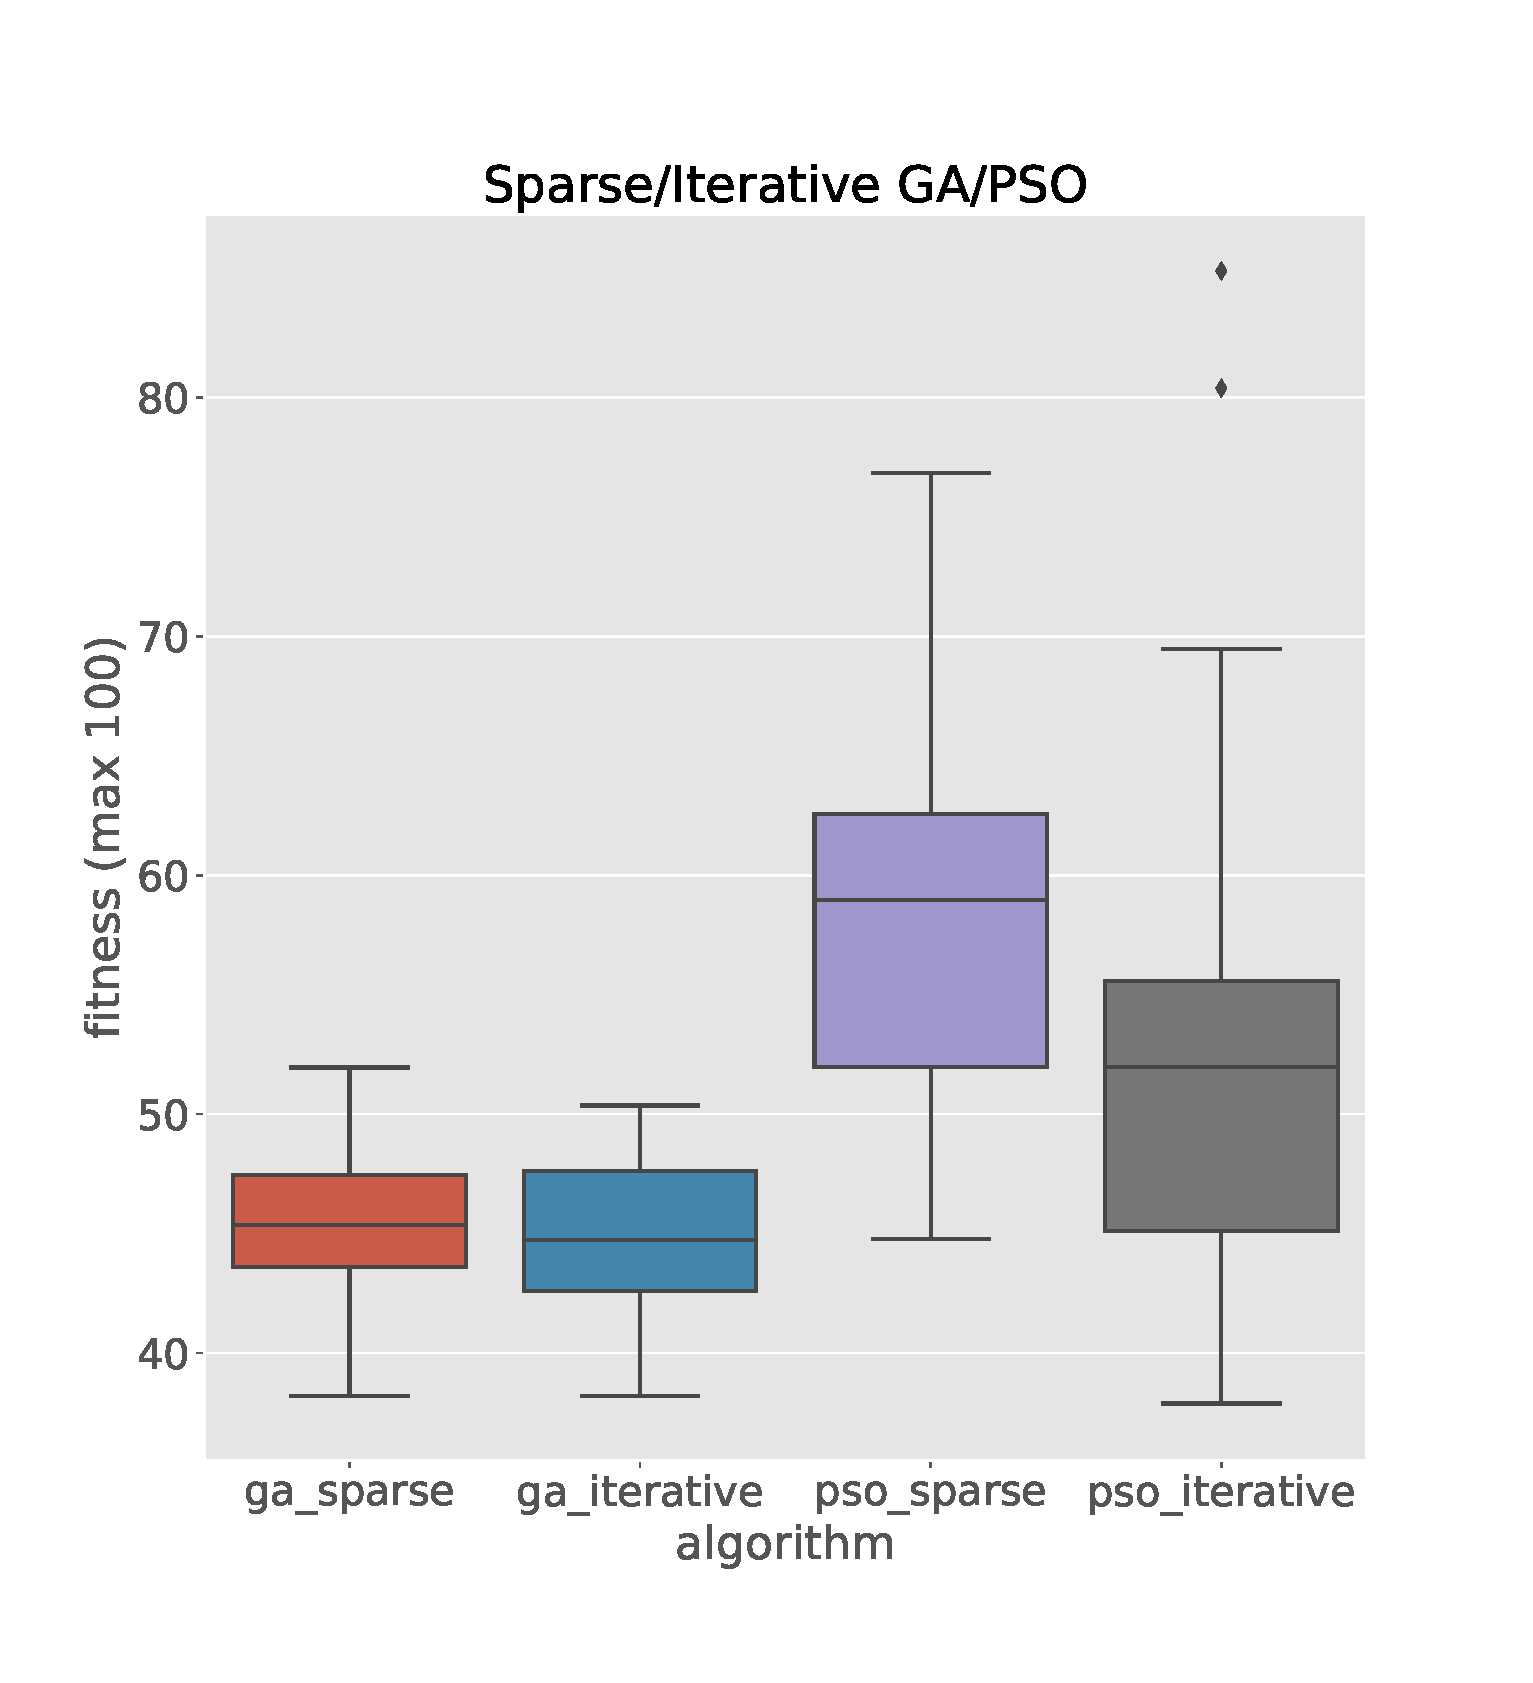
\includegraphics[width=0.5\textwidth]{old_images/overview.eps}
        \caption{The fitness comparison between the iterative and the sparse approached,
        both for the genetic algorithms and the PSO.  Difficulty: $5$.}
        \label{fig:overview}
    \end{figure}

    \begin{figure}[!ht]
        \centering
        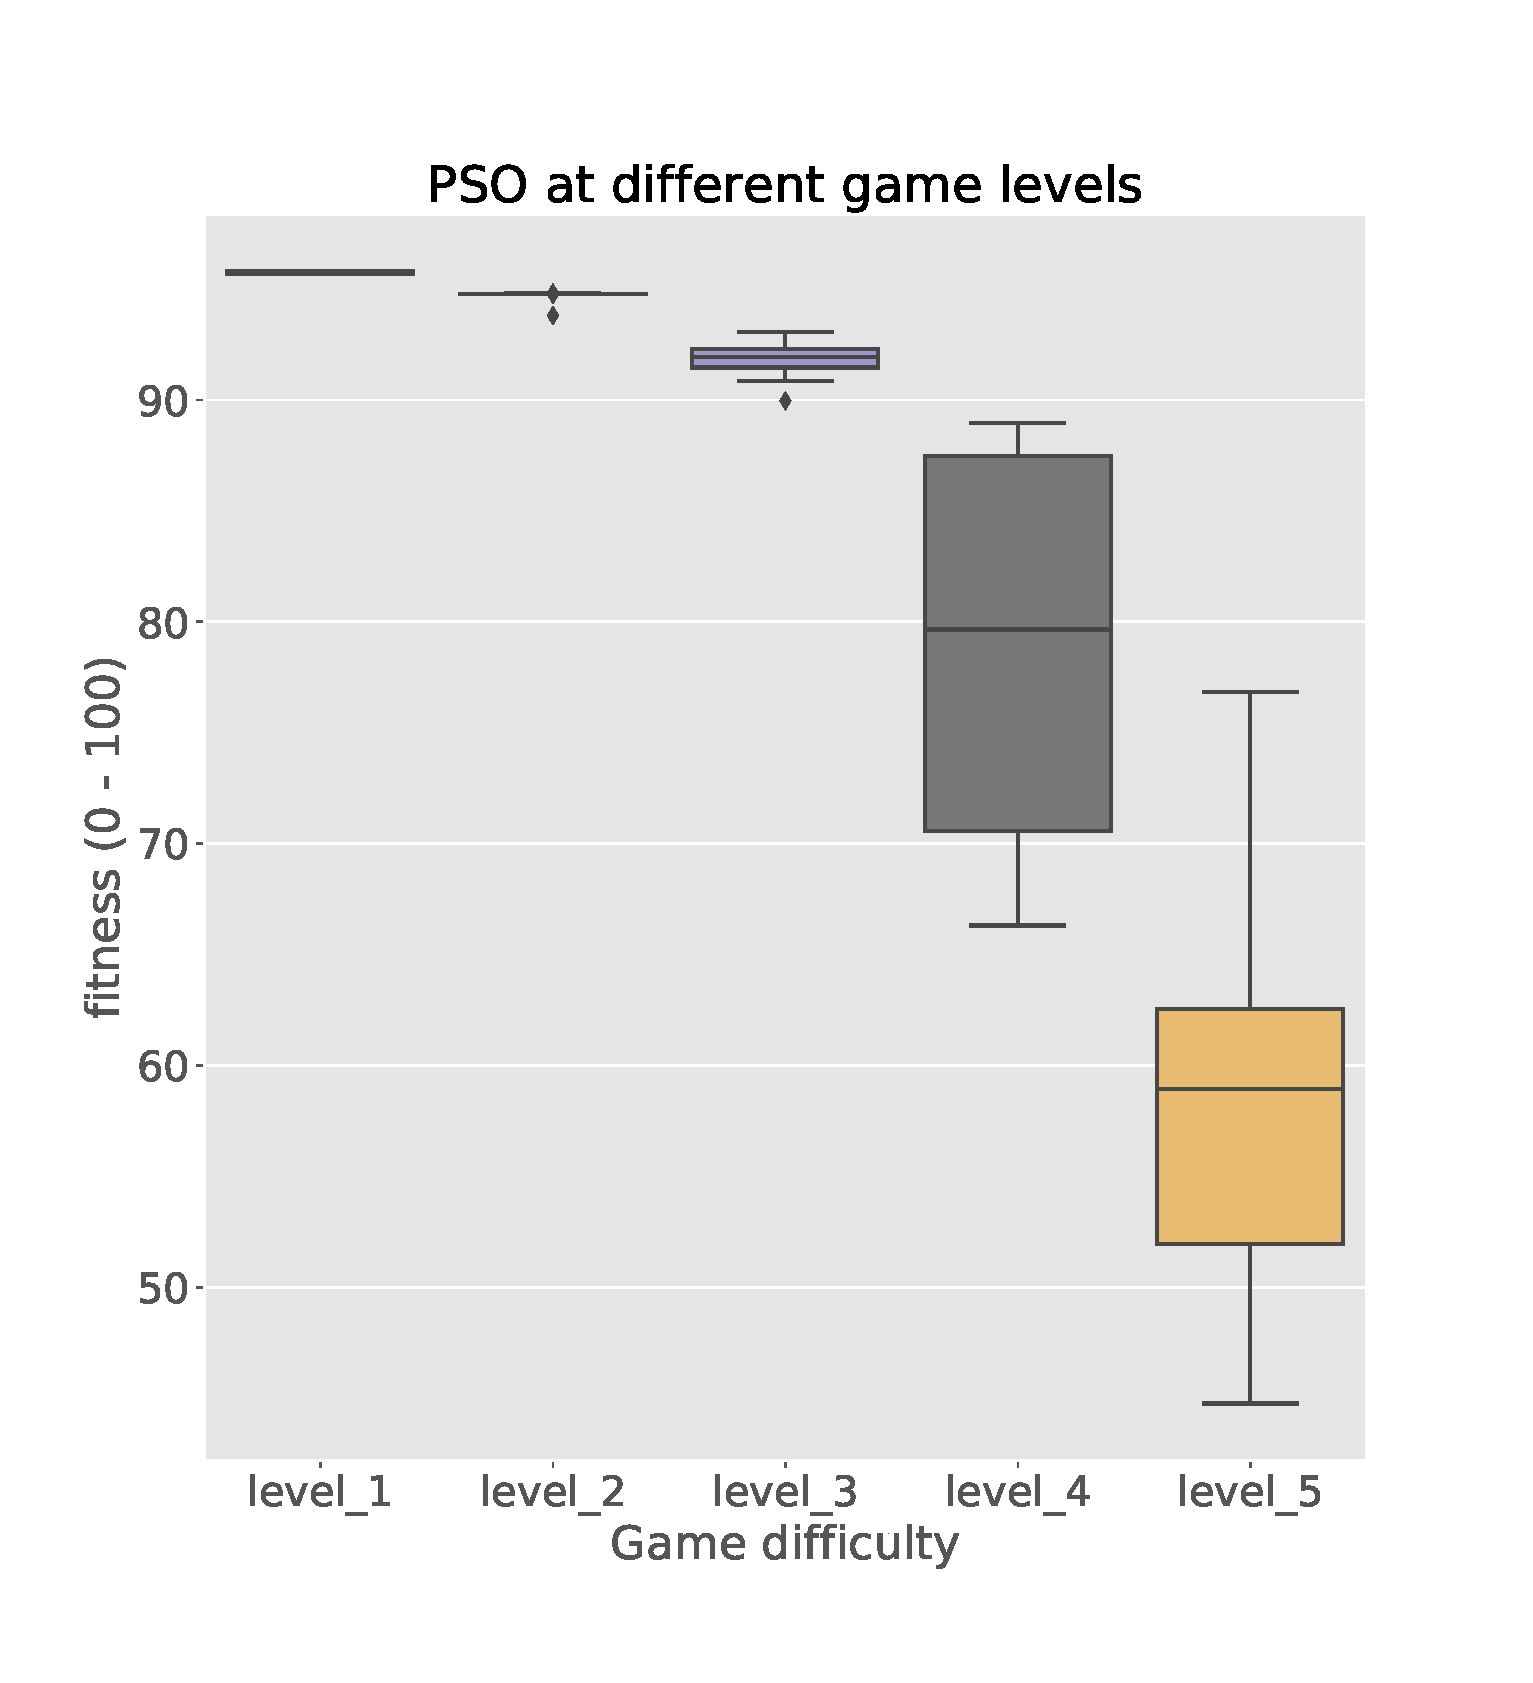
\includegraphics[width=0.5\textwidth]{old_images/pso_levels.eps}
        \caption{The fitness comparison of PSO against different game difficulty levels.}
        \label{fig:pso_levels}
    \end{figure}

  %    \phantom{ }
    
    
    \section{Initial Results}\label{sec:results}
    For evaluating an agent, we ran $30$ games against each opponent,
    leading to $8$ averages ($1$ per opponent), of which we computed the harmonic mean,
    which is the final result for the agent.
    We use the harmonic mean because it is used for reporting other results for this problem\cite{evoman_competition}.

    \subsection{Best Combination of Opponents for Training}\label{subsec:best-combination-of-opponents-for-training}
    We searched for the best $4$ opponents to serve as a basis for generalization.
    The first subset considered was $\{1, 2, 6, 7\}$, which was chosen empirically after manually playing against every opponent. We choose the ones which exhibited the most general behaviors our agents could learn, in our opinion. We performed a non-exhaustive search, and found no other $4$-opponent subset better than the human-chosen one.

    \subsection{Random Initialization PPO vs Cascading PSO $+$ PPO}\label{subsec:random-initialization-ppo-vs-pso-cascading-ppo}
    The best PSO configuration was used in cascade before the PPO in $4$ runs.
    PPO with random initialization was ran $3$ times.
    The small number of runs is due to the long training time.
    The worst result of the PPO with random initialization is far better than the best result
    of PSO cascaded with PPO\@, and we used this large difference to guide our choice, despite the small sample size. (Fig.~\ref{fig:random_vs_pso_initialization}).
    \begin{figure}[htbp]
        \centering
        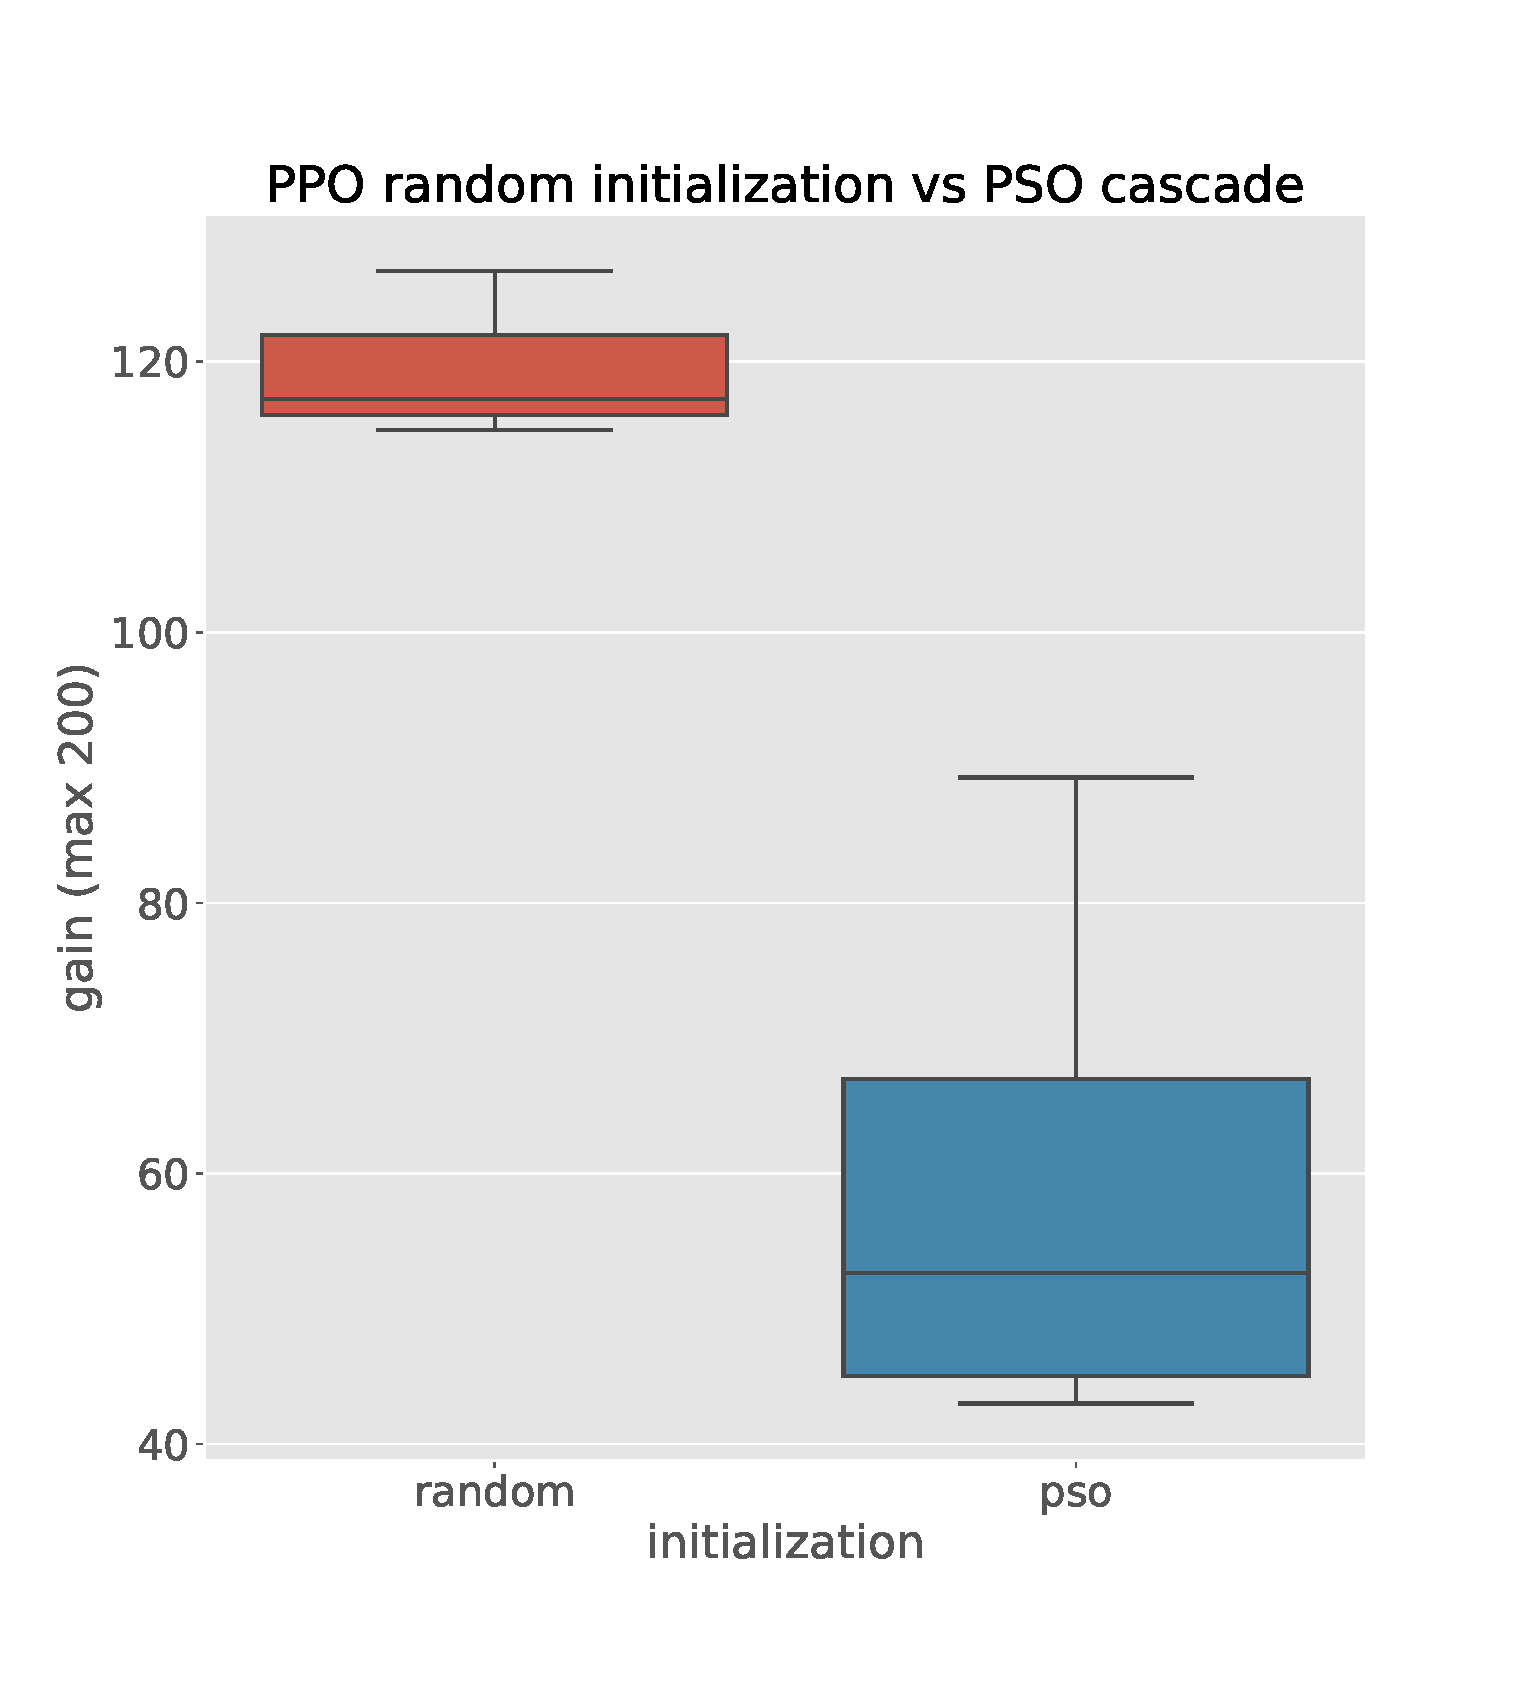
\includegraphics[width=0.5\textwidth]{images/random_vs_pso_initialization.eps}
        \caption{Gain comparison between PPO with random initialization and with PSO cascading.}
        \label{fig:random_vs_pso_initialization}
    \end{figure}

    \subsection{PPO in the best configuration}\label{subsec:ppo-on-the-best-configuration}
    Considering the results above, we decided that PPO with random initialization and training enemies $\{1, 2, 6, 7\}$ is the best configuration. We ran $3000$ epochs (chosen \textit{a priori}, considering only our experiences with PPO and general ANNs in other problems) in this configuration, saving all the models along the way after every $250$ epochs - since we anticipated overfit.
    \textit{After} looking at the testing results, we noticed that the final \textit{test} gain is greater after $2000$ epochs than after $3000$ epochs (Fig.\ref{fig:ppo_2000_vs_3000_epochs}).
    \begin{figure}[htbp]
        \centering
        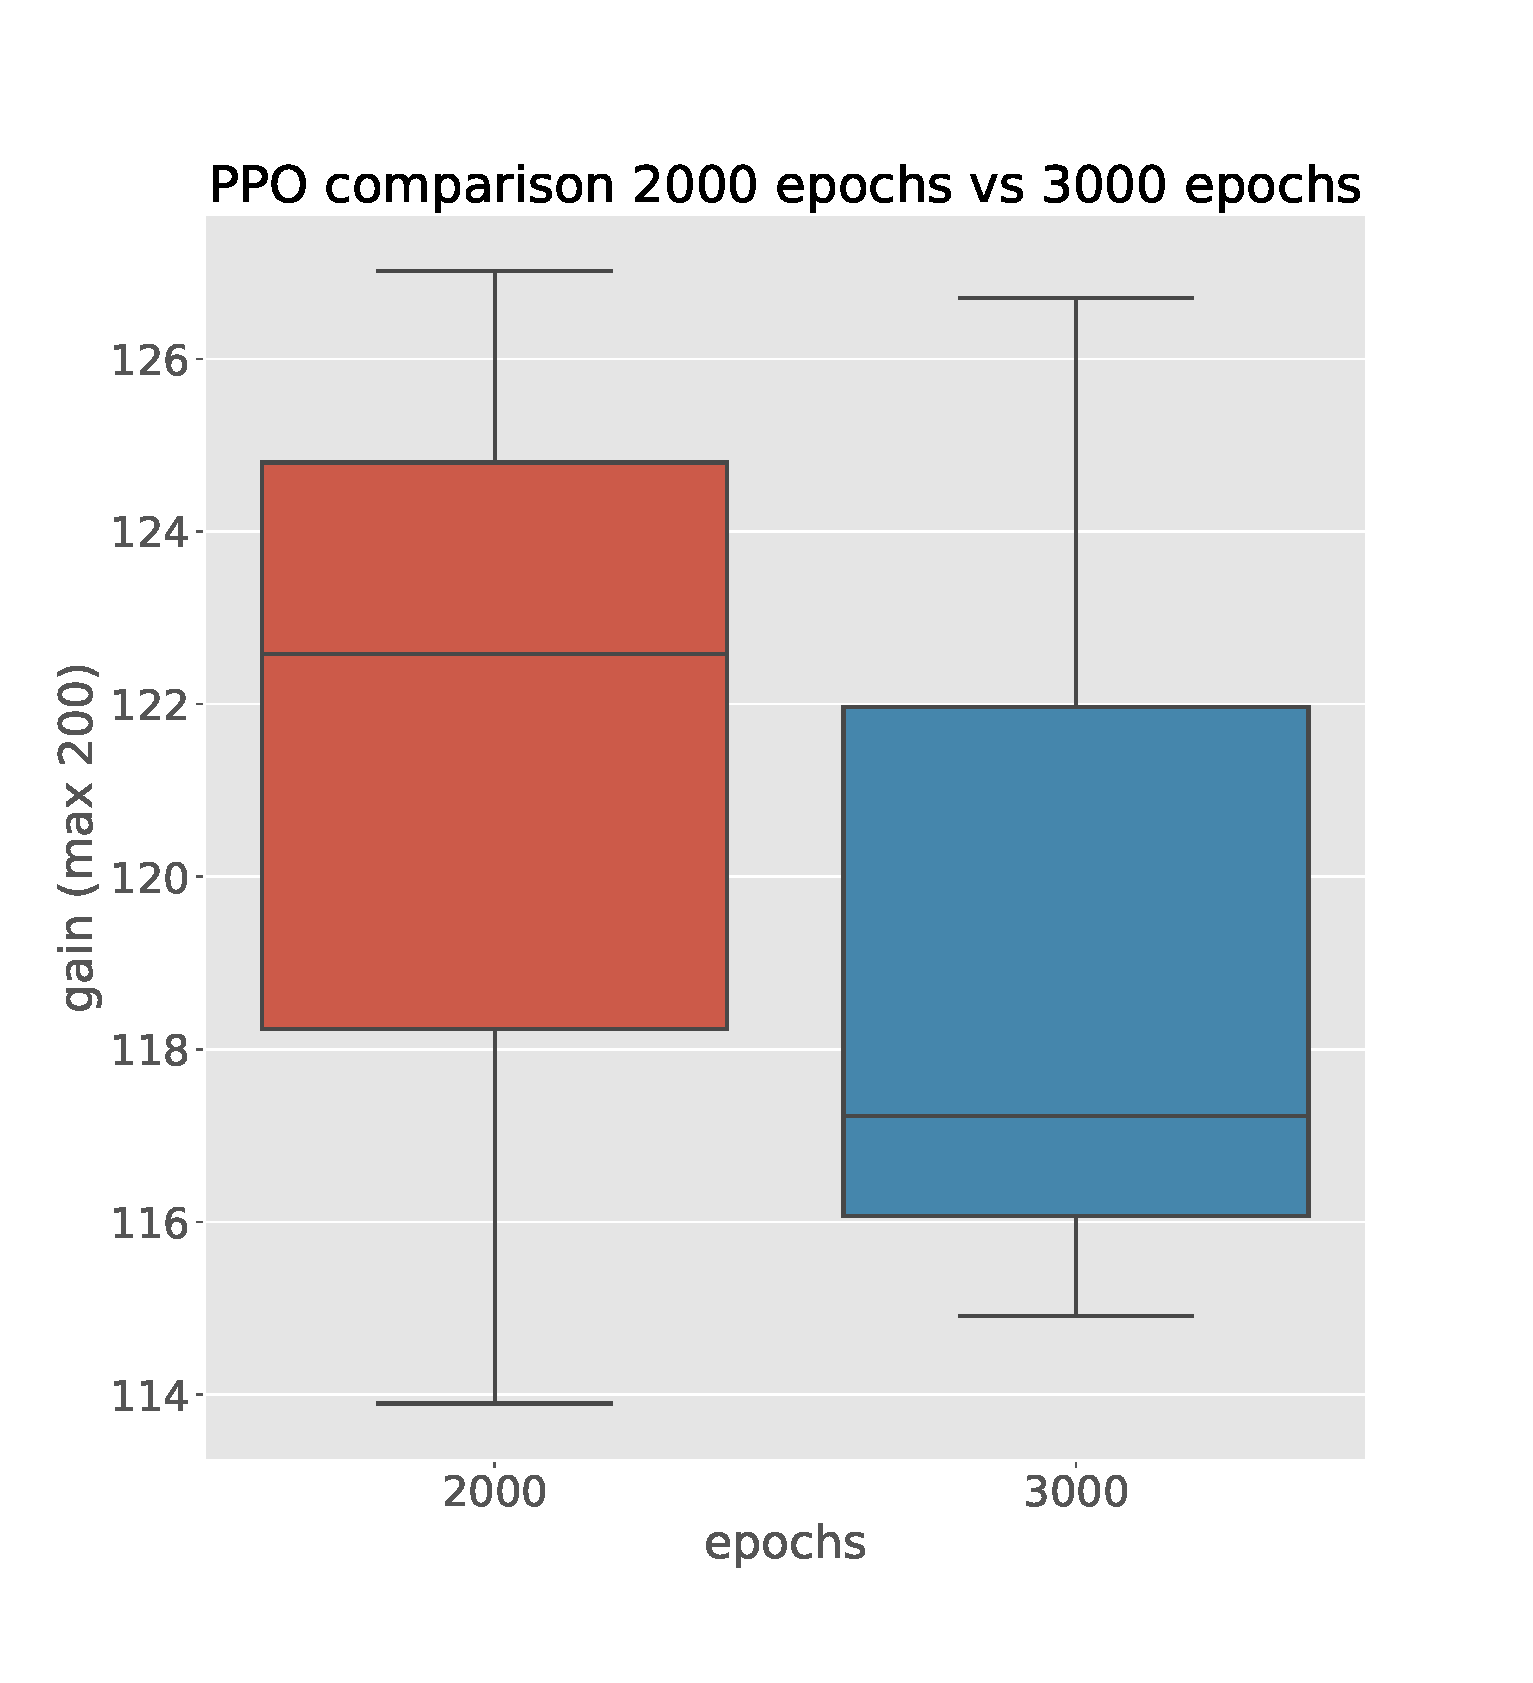
\includegraphics[width=0.5\textwidth]{images/ppo_2000_vs_3000_epochs.eps}
        \caption{Gain comparison between PPO after $2000$ epochs and after $3000$ epochs.}
        \label{fig:ppo_2000_vs_3000_epochs}
    \end{figure}



    \subsection{Best Train Agent vs Best Tested Agent}\label{subsec:best-tested-agent}
    The highest training gain is $198.4$.
    When computed against all opponents, this agent has an overall gain of $117.22$.
    Out of the $3$ PPO with random initialization runs, the highest test gain is $127.01$ (but they had lower training gains, due to overfit).
    After the experiments were concluded, we also looked at the overall gains of the agents before $3000$ epochs.
    The highest test gain was observed during the third run after $1750$ epochs, and it has a value of $137.18$.

    We were considerably computation-starved in these experiments; requiring a minimum sample size of $30$ meant we could only try out $3$ different agents. The competition organisers, upon running our algorithm, reported a different (and higher) value than in our experiments, of $138.14$ \cite{evoman_competition_results}.

    \begin{table}[htbp]
        \caption{Specialized NEAT vs Generalized PPO (Gain)}
        \begin{center}
            \begin{tabular}{|c|c|c|c|c|c|}
                \hline
                \textbf{Opponent}&\multicolumn{4}{|c|}{\textbf{PPO}}&\textbf{Specialized} \\
                \cline{2-5}
                & \textbf{\textit{Run 1}}& \textbf{\textit{Run 2}}& \multicolumn{2}{|c|}{\textbf{\textit{Run 3}}} & NEAT \\
                \cline{4-5}
                & $3000$ ep & $3000$ ep & $3000$ ep & $1750$ ep & \\
                & best train & & & best test & \\
                \hline
                $1$ & $198.41$ & $199.07$ & $199.81$ & $199.61$ & $190.01$ \\
                $2$ & $199.74$ & $199.27$ & $190.34$ & $189.14$ & $194.01$ \\
                $3$ & $58.94$  & $46.67$  & $70.27$  & $85.01$  & $180.01$ \\
                $4$ & $58.34$  & $66.5$   & $64.11$  & $80.17$  & $194.01$ \\
                $5$ & $172.61$ & $165.65$ & $174.61$ & $158.83$ & $194.01$ \\
                $6$ & $195.73$ & $196.95$ & $195.85$ & $194.37$ & $173.01$ \\
                $7$ & $199.79$ & $195.05$ & $193.27$ & $191.17$ & $177.01$ \\
                $8$ & $122.17$ & $145.49$ & $141.89$ & $140.61$ & $186.01$ \\
                \hline
              $\{1, 2, 6, 7\}$ & $198.4$ & $197.57$ & $194.75$ & $193.49$ & $183.09$ \\
              \hline
              $\{1,\dots,8\}$  & $117.22$ & $114.91$ & $127.01$ & $137.18$ & $185.67$ \\
              \hline
            \end{tabular}
            \label{tab1}
        \end{center}
    \end{table}


    \begin{table}[htbp]
        \caption{Specialized NEAT vs Generalized PPO (Percentage of games lost)}
        \begin{center}
            \begin{tabular}{|c|c|c|c|c|}
                \hline
                \textbf{Opponent}&\multicolumn{4}{|c|}{\textbf{PPO}} \\
                \cline{2-5}
                & \textbf{\textit{Run 1}}& \textbf{\textit{Run 2}}& \multicolumn{2}{|c|}{\textbf{\textit{Run 3}}} \\
                \cline{4-5}
                & $3000$ ep & $3000$ ep & $3000$ ep & $1750$ ep\\
                & best train & & & best test \\
                \hline
                $1$ & $0$     & $0$    & $0$     & $0$   \\
                $2$ & $0$     & $0$    & $0$     & $0$   \\
                $3$ & $96.67$ & $100$  & $96.67$ & $53.3$ \\
                $4$ & $100$   & $93.3$ & $100$   & $93.3$  \\
                $5$ & $0$     & $3.3$  & $0$     & $0$   \\
                $6$ & $0$     & $0$    & $0$     & $0$   \\
                $7$ & $0$     & $6.67$ & $0$     & $0$   \\
                $8$ & $20$    & $0$    & $3.3$   & $10$    \\
                \hline

            \end{tabular}
        \end{center}
    \end{table}

%    \begin{table}[!htbp]
%        \caption{Average player and enemy life. Average game duration (in frames)}
%        \begin{center}
%            \begin{tabular}{|c|c|c|c|c|c|c|}
%                \hline
%                \textbf{Opp}&\multicolumn{3}{|c|}{\textbf{Best train agent}}&\multicolumn{3}{|c|}{\textbf{Best test agent}} \\
%                \cline{2-7}
%                & \textbf{\textit{pl. life}}& \textbf{\textit{opp. life}}& \textbf{\textit{frames}} & \textbf{\textit{pl. life}}& \textbf{\textit{opp. life}}& \textbf{\textit{frames}} \\
%              \hline
%              1 & 97.26 &     0 &  159.63 &    100 &     0 &  174.23 \\
%              2 & 98.33 &     0 &   176.6 &  89.73 &     0 &  186.43 \\
%              3 &  0.13 & 43.33 &  457.26 &   7.66 & 21.33 &  410.53 \\
%              4 &     0 & 37.66 &   547.5 &   1.84 & 21.66 &  736.83 \\
%              5 & 71.32 &     0 &  379.13 &  60.52 &     0 &  367.93 \\
%              6 & 96.32 &     0 &  165.06 &     95 &     0 &  203.53 \\
%              7 & 99.74 &     0 &  162.06 &   85.9 &     0 &  135.13 \\
%              8 &  34.3 &     6 &  520.93 &  38.76 &     2 &   443.6 \\ \hline
%              \textbf{Avg} & 62.17 & 10.87 & 321.02 & 59.92 & 5.62 & 332.27 \\
%              \hline
%            \end{tabular}
%        \end{center}
%    \end{table}



    \section{Increasing the Upper Bound}\label{subsec:increasing-the-upper-bound}
    Our PPO implementation wasn't able to generalise sufficiently, neither in the competition (where our gain of $138.14$ was below the best gain of $146.88$)\cite{evoman_competition_results}, nor in our own tests. Overfitting was a significant problem, and we believe it to be a good indicator of our issues.
    
    However, with the PPO trained on opponents $\{1, 2, 6, 7\}$, we have surpassed the best specialised opponent-specific models from the original paper, which were given as upper bounds\cite{evoman}. Thus, we can understand this issue as an exploration versus exploitation trade-off: while we haven't been able to develop the best exploratory, generalising model, we seem to have found a very good exploitative, targeted solution.

    As such, we've performed $3$ further experiments which:
    \begin{itemize}
    \item develop a unified model for opponents $\{1, \dots, 8\}$, training on opponents $\{1, \dots, 8\}$, at difficulty $2$.
    \item develop a unified model for opponents $\{1, \dots, 8\}$, training on opponents $\{1, \dots, 8\}$, at difficulties $\{1, \dots, 5\}$.
    \item develop individual models for each opponent, training on each respective opponent, at difficulty $2$.
    \end{itemize}

    We shall call the unified model ``generalised'' and the individual model(s) ``specialised''.

    Beyond these changes in aim, we haven't modified the above-described PPO algorithm employed.

    \subsection{Single difficulty}
    
    \begin{table}[htbp]
        \caption{PPO generalised vs PPO specialised vs NEAT specialised, difficulty $= 2$}
        \begin{center}
            \begin{tabular}{|c|c|c|c|}
                \hline
                \textbf{Opponent}&\textbf{PPO gen.}&\textbf{PPO spec.}&\textbf{NEAT spec.} \\
                \hline
                 1 &  199.54 &  199.67 &  190.01 \\
                 2 &  200.01 &  199.61 &  194.01 \\
                 3 &  194.81 &  199.94 &  180.01 \\
                 4 &  180.61 &  195.95 &  194.01 \\
                 5 &  187.77 &  198.03 &  194.01 \\
                 6 &  174.43 &  199.67 &  173.01 \\
                 7 &  183.07 &  197.73 &  177.01 \\
                 8 &  169.31 &  195.07 &  186.01 \\
                \hline
                \textbf{harmonic mean} & 185.57 & 198.19 & 185.67 \\
                \hline
            \end{tabular}
            \label{PPO generalized vs specialized vs NEAT}
        \end{center}
    \end{table}    

    The specialised PPO was able to surpass the specialised NEAT\cite{evoman} algorithm, both in harmonic mean and in each individual case (Table \ref{PPO generalized vs specialized vs NEAT}). The specialised PPO agents were trained for $1000$ epochs, as they achieved excellent results.

    Additionally, PPO was able to create a general model which is extremely close (a $0.1$ gain difference) in harmonic mean to the results of the $8$ specialised models evolved through NEAT.
    
    \subsection{Multiple difficulties}

    \begin{figure}[htbp]
    \centering
    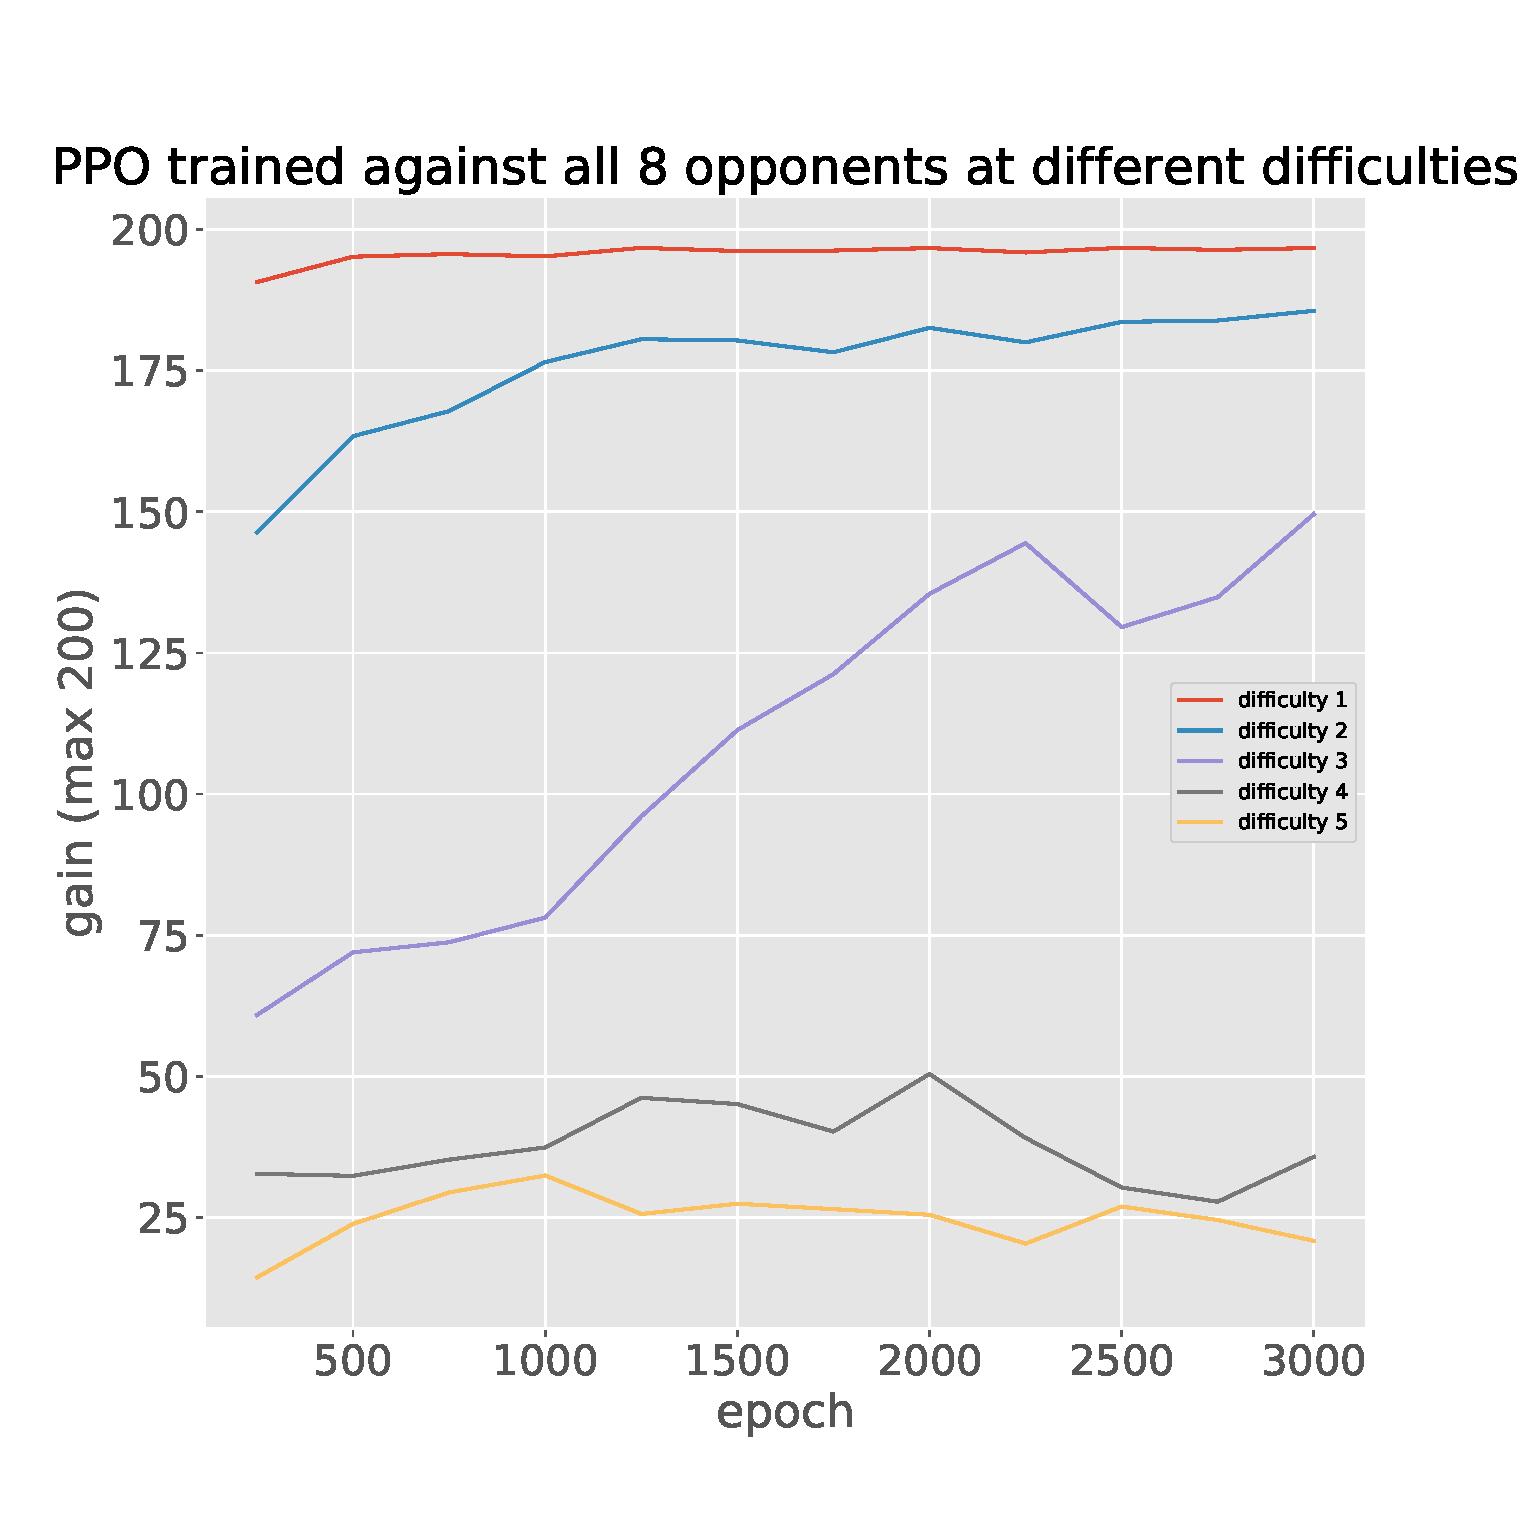
\includegraphics[width=0.5\textwidth]{images/general_harmonic_gain.eps}
    \caption{Gain Evolution for PPO when trained against all 8 opponents. (In case of grayscale viewing: the plots are fully sorted, with difficulty $1$ being the highest, and difficulty $5$ the lowest.)}
    \label{fig:ppo_train_8}
    \end{figure}

    \begin{table}[htbp]
        \caption{PPO (generalised) trained against all opponents (Gain)}
        \begin{center}
            \begin{tabular}{|c|c|c|c|c|c|}
                \hline
                \textbf{Opponent}&\multicolumn{5}{|c|}{\textbf{Difficulty}} \\
                \cline{2-6}
                & \textbf{\textit{1}}& \textbf{\textit{2}}& \textbf{\textit{3}} & \textbf{\textit{4}} & \textbf{\textit{5}} \\
                \hline
                 1 &  200.01 &  199.54 &  170.75 &  155.48 &   41.08\\
                 2 &  200.01 &  200.01 &  182.81 &  168.81 &  168.51\\
                 3 &  199.38 &  194.81 &  164.31 &  127.54 &  130.61\\
                 4 &  186.14 &  180.61 &  154.23 &  181.58 &   60.28\\
                 5 &  196.56 &  187.77 &  185.34 &  142.41 &  158.31\\
                 6 &  196.35 &  174.43 &  179.19 &   23.84 &    9.88\\
                 7 &  199.26 &  183.07 &   95.40 &    8.01 &    8.28\\
                 8 &  196.57 &  169.31 &  123.00 &   41.34 &   10.01\\
                \hline
                \textbf{harmonic mean} & 196.68 & 185.57 & 149.57 & 35.76 & 20.89 \\
                \hline
            \end{tabular}
            \label{PPO against all opponents gain}
        \end{center}
    \end{table}


    \begin{table}[htbp]
      \caption{PPO (specialised), trained $1000$ epochs (gain)}
              \begin{center}
            \begin{tabular}{|c|c|c|c|c|}
                \hline
                \textbf{Opponent} & \multicolumn{4}{|c|}{\textbf{Difficulty}} \\
                \cline{2-5}
                & \textbf{\textit{2}} & \textbf{\textit{3}} & \textbf{\textit{4}} & \textbf{\textit{5}} \\
                \hline
                1                      & 199.68              & 196.51              & 189.21              & 166.01              \\
                2                      & 199.61              & 199.91              & 199.21              & 197.18              \\
                3                      & 199.94              & 199.51              & 147.21              & 72.28               \\
                4                      & 195.95              & 196.14              & 198.81              & 191.23              \\
                5                      & 198.03              & 193.38              & 191.73              & 196.71              \\
                6                      & 199.67              & 195.18              & 196.85              & 198.76              \\
                7                      & 197.73              & 192.45              & 184.85              & 176.01              \\
                8                      & 195.07              & 185.37              & 178.05              & 172.61              \\
                \hline
                \textbf{harmonic mean} & 198.19              & 194.7               & 184.12              & 154.58              \\
                \hline
            \end{tabular}
            \label{Specialized PPO against multiple difficulties (gain)}
        \end{center}
        \end{table}
    
    \begin{table}[htbp]
        \caption{PPO - percentage of games lost}
        \begin{center}
            \begin{tabular}{|c|c|c|c|c|c|c|c|c|c|}
                \hline
              \textbf{Opp.}&\multicolumn{9}{|c|}{\textbf{Difficulty}} \\
              \cline{2-10}
                           & \multicolumn{5}{|c|}{Generalised} & \multicolumn{4}{|c|}{Specialised} \\
              \cline{2-10}
                & \textbf{\textit{1}}& \textbf{\textit{2}}& \textbf{\textit{3}} & \textbf{\textit{4}} & \textbf{\textit{5}} & \textbf{\textit{2}}& \textbf{\textit{3}} & \textbf{\textit{4}} & \textbf{\textit{5}}\\
                \hline
                 1 &  0 &  0 &     20 &  23.33 &   100 & 0 & 0 & 0     & 13.33 \\
                 2 &  0 &  0 &      0 &      0 &     0 & 0 & 0 & 0     & 0 \\
                 3 &  0 &  0 &      0 &  13.33 &  3.33 & 0 & 0 & 36.67 & 100 \\
                 4 &  0 &  0 &      0 &      0 &    60 & 0 & 0 & 0     & 0 \\
                 5 &  0 &  0 &      0 &      0 &     0 & 0 & 0 & 0     & 0 \\
                 6 &  0 &  0 &      0 &    100 &   100 & 0 & 0 & 0     & 0 \\
                 7 &  0 &  0 &  56.66 &    100 &   100 & 0 & 0 & 0     & 0 \\
                 8 &  0 &  0 &     10 &    100 &   100 & 0 & 0 & 0     & 0 \\
                \hline
            \end{tabular}
            \label{PPO against all opponents games lost}
        \end{center}
    \end{table}

    Since our generalised PPO model is very close to the previous upper bound, we believe our single-model, all-opponent, all-difficulty exploration should provide a good estimation of what constitutes a good result on all difficulty levels.

    At difficulty $5$, with opponent-specific models (Table \ref{Specialized PPO against multiple difficulties (gain)}) we also establish a good upper bound. $4$ opponents are easily defeated, and a single opponents proves difficult.
  
    \section{Conclusions}\label{sec:conclusions}
    \subsection{Upper Bound}
    As stated previously, interpreting the initial issue as an exploration versus exploitation trade-off allowed us to repurpose the PPO algorithm. While it wasn't neither exploratory nor flexible enough to provide the best generalisation from $4$ opponents to $8$, it was exploitative enough to significantly increase the opponent-specific upper bound.
   
    Even with a more modest $1000$-epoch runtime, the specialised PPO is able to easily exceed the previous upper bound\cite{evoman}, and approach the maximum gain of $200.01$. In fact, it does so for opponent $2$, apparently the easiest for our algorithm to defeat, according to Table \ref{PPO against all opponents gain}.

    This previous upper-bound was established with a specialised (one model per opponent) NEAT algorithm, and we feel the comparison is fair: matching specialised algorithm to specialised algorithm.

    While the previous upper bound does not have a time estimate attached to it, given our experience with both methods, we believe our proposed algorithm to be slower than NEAT, due to NEAT's ability to change, and minimse, the structure of the evolved ANN, and its ability to make larger exploratory jumps. For instance, establishing specialised upper bounds for each difficulty (Table \ref{Specialized PPO against multiple difficulties (gain)}) required $10$ million Evoman frames (accumulated during $1000$ training epochs) per opponent, per difficulty level.

    The single-model, all-opponent PPO seems to match the previous upper bound; given the gain range of $[0, 200.01]$, and the range the results take values in, we believe that a difference of $0.1$ is not significant. Thus, we show that a single model can perform very well against all $8$ opponents (how an algorithm might generalise such a model from fewer opponents to all opponents remains an open, difficult problem).

    We feel this is an important result: while the initial upper bound\cite{evoman} provided $8$ separate models to deal with $8$ opponents, we show that there exists a single model which is, in harmonic mean, just as good. We also believe that there is room for improvement for opponent-generalising algorithms. For the first statement, we have proof-by-existence: if our PPO found the model, then it most certainly exists, and is possible to achieve through other algorithms. The second statement - belief - we cannot prove yet; it would require showing that the behaviour patterns learned on one opponent can be applied to others, to a very high degree.

    \subsection{Other Difficulty Levels}
    In both our PSO (Fig. \ref{fig:pso_levels}) and PPO (Table \ref{PPO against all opponents gain}) explorations, we have found the game difficulty to matter a great deal. The generalised PPO, while inferior to the opponent-specialised PPO models in most cases, does establish the upper bound for opponent $3$ (Tables \ref{PPO against all opponents gain} and \ref{Specialized PPO against multiple difficulties (gain)}).

    We'd like to propose difficulty $3$ as an interesting problem in itself. As shown in Fig. \ref{fig:ppo_train_8}, PPO shows the greatest improvement there, from the first to the last epoch. Difficulties $1$ and $2$ are  easier to solve, while $4$ and $5$ are currently very difficult - but all $4$ show relatively flat improvement curves. Algorithms playing Evoman at difficulty $3$ could show the greatest variance in results and further guide our algorithm-crafting decisions.

    \subsection{Future Work}

    We believe that, given the difficulty of the generalisation problem, pushing for greater exploration, while retaining our current level of exploitation are both required. We've attempted this with the $2$-stage cascade ensemble method, but we believe now that separating the exploratory and exploitative stages was a mistake (guided by our limited computational resources). The game is too difficult for the best strategies to be \textit{local} refinements of simple strategies. In other words, our results show that the function landscape contains multiple wider, shallower strictly-local optima basins, while the attraction basins for global optima are deep and narrow. There is also a degree of optimum dynamics: opponents don't perform the same recipe of actions, but have a limited ability to react to our agent / player.

    Retaining the current level of exploration, while increasing exploitation can be done by greatly increasing the computational resources allocated to solving the problem\cite{nfl}. Based on our results (Fig. \ref{fig:overview}), we recommend a PSO$+$PPO Memetic Algorithm\cite{memetic}. 

    A way to sidestep the increase in computational time could be creating an on-line learning algorithm / agent. Thinking about the problem as a prediction problem - ``if half the opponents behaved in their certain ways, how will the rest behave? '' - , we can have $2$ basic ways of dealing with the prediction. 

    
%\vfill\null
    
%\pagebreak

    
    We can try to predict the full behaviour of the remaining test opponents ahead of time, or we can try to predict each action-by-action, as we confront them. Despite the increase in algorithmic difficulty for on-line learning, the second problem seems far easier than the first. Building on the previous proposal, we'd advise a sparse PSO$+$PPO Memetic Algorithm. While sparse PPO didn't achieve better results in our exploratory tests, they were evaluated only on basic (simpler, and requiring fewer computational resources) strategies. 

     

    \section{Acknowledgments}
    We'd like to thank the creators and developers of Evoman for their implementation and documentation efforts. We'd also like to thank Ioana-Teodora Norocea for her editing help.

    \begin{thebibliography}{00}
    \bibitem{evoman_competition} Evoman: Game-playing Competition for WCCI 2020, \url{http://pesquisa.ufabc.edu.br/hal/Evoman.html}
    \bibitem{evoman_competition_results} Evoman: Game-playing Competition for WCCI 2020, results \url{http://pesquisa.ufabc.edu.br/hal/Evoman.html#results}
    \bibitem{evoman} Fabricio Olivetti de Franca, Denis Fantinato, Karine Miras, A.E. Eiben and Patricia A. Vargas.
      "EvoMan: Game-playing Competition" arXiv:1912.10445
    \bibitem{karinemiras} de Araújo, Karine da Silva Miras, and Fabrício Olivetti de França.
      "An electronic-game framework for evaluating coevolutionary algorithms." arXiv:1604.00644 (2016).
    \bibitem{neuro} Floreano, D., Dürr, P. \& Mattiussi, C. Neuroevolution: from architectures to learning. Evol. Intel. 1, 47–62 (2008). \url{https://doi.org/10.1007/s12065-007-0002-4}
    \bibitem{capcom} M. MEGA, "Produced by capcom, distributed by capcom, 1987," System: NES.
    \bibitem{q_learning} Watkins, C.J.C.H., Dayan, P. Q-learning. Machine Learning 8, 279–292 (1992)
    \bibitem{genetic_algorithm} Holland J.H., Genetic Algorithms and Adaptation. Adaptive Control of Ill-Defined Systems, 1984, Volume 16 ISBN 978-1-4684-8943-9
    \bibitem{pso} Kennedy, J.; Eberhart, R. (1995). "Particle Swarm Optimization". Proceedings of IEEE International Conference on Neural Networks. IV. pp. 1942–1948.
    \bibitem{neat} Kenneth O. Stanly; Rist Miikkulainen (2002). "Evolving Neural Networks through Augmenting Topologies". Evolutionary Computation, Volume 10, Issue 2, Summer 2002, p.99-127, \url{https://doi.org/10.1162/106365602320169811}
    \bibitem{ppo} John Schulman, Filip Wolski, Prafulla Dhariwal, Alex Radford, Oleg Klimov (2017) "Proximal Policy Optimization Algorithms", arXiv:1707.06347v2
    \bibitem{memetic} Moscato, P. (1989). "On Evolution, Search, Optimization, Genetic Algorithms and Martial Arts: Towards Memetic Algorithms". Caltech Concurrent Computation Program (report 826).
    \bibitem{cybenko} Cybenko, G. (1989). "Approximations by superpositions of sigmoidal functions", Mathematics of Control, Signals, and Systems, 2(4), 303–314. doi:10.1007/BF02551274
    \bibitem{nfl} Wolpert, D.H., Macready, W.G. (1997), "No Free Lunch Theorems for Optimization", IEEE Transactions on Evolutionary Computation 1, 67.
    \bibitem{evoman_blog} Karine Miras, Evoman, \url{https://karinemirasblog.wordpress.com/portfolio/evoman/}
    \bibitem{spinningUp} Joshua Achiam, 2018, ``Spinning Up in Deep Reinforcement Learning'' \url{https://github.com/openai/spinningup}
    \end{thebibliography}

\end{document}



